% Document
% Document
\documentclass[12pt, a4paper]{article}
\usepackage[T1]{fontenc}
\usepackage[utf8]{inputenc}
\usepackage{authblk}
\usepackage{lipsum}
\usepackage{tikz}
\usepackage{hyperref}

% Figure and table formating
\usepackage{epsfig}
\usepackage{tabu}
\usepackage{rotating}
\usepackage{pbox}
\usepackage{framed, multicol}
\usepackage[framemethod=TikZ]{mdframed}

% Set up Frame
\mdfdefinestyle{MyFrame}{%
    linecolor=black,
    skipabove=10pt,
    outerlinewidth=2pt,
    roundcorner=20pt,
    innertopmargin=10pt,
    innerbottommargin=10pt,%\baselineskip,
    innerrightmargin=20pt,
    innerleftmargin=20pt,
    backgroundcolor=gray!50!white}

\usepackage{float}
\usepackage[left=1 in, right=1 in, top=1.25 in, bottom=1.25 in]{geometry}

% Fonts - Mathtime
%\usepackage{txfonts}
\usepackage{amsmath} % Add amssymb if not using Mathtime

% Text
\setlength{\parindent}{0.5in}
\frenchspacing  \tolerance = 800  \hyphenpenalty = 800

\usepackage{lineno} % Line numbers
\def\linenumberfont{\normalfont\footnotesize\ttfamily}
\setlength\linenumbersep{0.1 in}

\usepackage{setspace}

% Format section and subsection headers
\makeatletter
\renewcommand{\section}{\@startsection
{section}%                   % the name
{1}%                         % the level
{0mm}%                       % the indent
{-\baselineskip}%            % the before skip
{0.5\baselineskip}%          % the after skip
{\normalfont\bf\large}} % the style

\renewcommand{\subsection}{\@startsection
{subsection}%                   % the name
{2}%                         % the level
{0mm}%                       % the indent
{-\baselineskip}%            % the before skip
{0.5\baselineskip}%          % the after skip
{\normalfont\bf}} % the style
\makeatother

% Other
\usepackage{graphicx}
\usepackage[singlelinecheck=false,font=small,labelfont=bf]{caption}

% Bibliography
\usepackage[numbers, compress]{natbib} % Bibliography - APA
\bibpunct{(}{)}{;}{a}{}{,}

% Format the Bibliography appropriately
% increase \bibhang to take care of the numbers
% \setlength{\bibhang}{0pc}
% \makeatletter
% % patch \@lbibitem to print the current number before the authors
% \patchcmd{\@lbibitem}
%   {]}
%   {] \theNAT@ctr. \newline }
%   {}{}
% \makeatother


%%%%%% FRONT MATTER %%%%%%%%%

\begin{document}

% \begingroup
\setlength{\parindent}{0in}
\renewcommand{\arraystretch}{2}
% \renewcommand{\tabcolsep}{0}
%\renewcommand{\tabrowsep}{1}
\begin{tabular}{p{3cm} p{10cm}}

\large\textbf{} & \vspace\baselineskip \\

\textbf{Title:} & Detecting and quantifying parasite-induced host mortality from intensity data: method comparisons and limitations \\

\textbf{Running title:} & Methods for quantifying parasite-induced host mortality  \\

\textbf{Authors:} & Mark Q. Wilber, Sara B. Weinstein and Cheryl J. Briggs \\

\textbf{Statement of Authorship:} & MW and SW designed research, performed
analyses and wrote the manuscript, CB designed research and contributed to revisions. \\

\textbf{Affiliations:} &
1) Department of Ecology, Evolution and Marine Biology, University of California,
Santa Barbara, Santa Barbara California, United States of America \\

\textbf{Email addresses:} &
Mark Wilber: mark.wilber@lifesci.ucsb.edu \newline
Sara Weinstein: sara.weinstein@lifesci.ucsb.edu \newline
Cheryl Briggs: cherie.briggs@lifesci.ucsb.edu \\

\textbf{Corresponding \newline author:} &
Mark Wilber \newline
University of California, Santa Barbara \newline
Department of Ecology, Evolution, and Marine Biology \newline
2111 Noble Hall \newline
Santa Barbara, CA 93106 \newline
505-321-5381 \newline
mark.wilber@lifesci.ucsb.edu \newline


\end{tabular}

\textbf{Note}: Supplementary data associated with this article


% \renewcommand{\arraystretch}{1}
% \begin{tabular}{l l}

% \textbf{Words - Abstract:} & 293 \\
% \textbf{Words - Main Text:} & 4988 \\
% \textbf{References:} & 50 \\
% \textbf{Figures:} & 5 \\
% \textbf{Tables:} & 1

% \end{tabular}

\newpage

\abstract{

Parasites can significantly impact animal populations by changing host
behavior, reproduction and survival. Detecting and quantifying these impacts is
critical for understanding disease dynamics and managing wild animal
populations. However, for wild hosts infected with macroparasites, it is
notoriously difficult to quantify the fatal parasite load and number of animals
that have died due to disease. When ethical or logistical constraints prohibit
experimental determination of these values, examination of parasite intensity
and distribution data may offer an alternative solution. In this study we
introduce a novel method for using intensity data to detect and quantify
parasite-induced mortality in wildlife populations. We use simulations to show
that this method is more reliable than previously proposed methods while
providing quantitative estimates of parasite-induced mortality from empirical
data that are consistent with previously published qualitative estimates.
However, this method, and all techniques that estimate parasite-induced
mortality from intensity data alone, have several important assumptions that
must be scrutinized before applying them to real-world data. Given that these
assumptions are met, our method is new exploratory tool that can help inform
more rigorous studies of parasite-induced host mortality.

\textbf{Keywords}: parasite aggregation, negative binomial distribution, Crofton Method, host survival function, lethal dose

}

\doublespacing

\linenumbers
\section{Introduction}

Infectious agents can impact animal populations by changing
population dynamics and stability \citep{Dobson1992,Tompkins2002}, altering predator-prey interactions \citep{Joly2004}, and
even causing species' decline and extinction \citep{DeCastro2005a,McCallum2012b}. Accurately estimating the impact
of these infectious agents in wildlife is critical to understanding what
regulates host and parasite populations, making predictions about disease
transmission, and managing disease outbreaks \citep{Langwig2015}. The impact of pathogens, such as rabies \citep{Coyne1989}, bovine tuberculosis \citep{Cox2005}, and
rinderpest \citep{Tille1991}, are typically modeled based on the presence or absence of disease, such that host survival is not typically considered to be a function of the number of infectious agents present within the host.  In contrast, models of macroparasites generally assume that pathology increases with parasite burden and host survival probability must be treated as a function of infection intensity \citep{AndersonandMay1978}. Helminths exhibiting this intensity-dependent pathology have significant impacts on human health \citep{Brooker2004}, domestic livestock economics \citep{Roeber2013}, and wildlife survival \citep{Kirk2003,Logiudice2003}. While it is generally assumed that some fraction of wild host populations succumb to parasitic infection, it is notoriously difficult to actually quantify parasite-induced host mortality (PIHM) in wild animal populations because it is difficult to observe the dead or dying hosts most impacted by parasitism \citep{McCallum2000a}.

Ideally, parasite-induced host mortality is
quantified by experimentally infecting and tracking individual hosts in the
wild population; however, for logistical and ethical reasons this method is
rarely feasible \citep{McCallum2000a}. Snapshot data of parasite intensities across multiple hosts is much easier to collect and has
often been used to identify the presence of PIHM \citep{Crofton1971a,Lester1977,Lester1984,Lanciani1989,Royce1990,Ferguson2011} and to quantify the
relationship between infection intensity and host mortality \citep{Adjei1986}.

\cite{Crofton1971a} first proposed that PIHM could be identified from parasite intensity data by comparing the
observed parasite distribution in sampled hosts to the distribution
predicted in the absence of parasite-induced mortality. This method
assumes that, prior to host mortality, infection intensity in the host population follows a negative binomial distribution and the tail of the distribution is truncated as intensity dependent pathology removes the most heavily infected hosts. Assuming mortality occurs only in heavily infected hosts, evidence of this parasite-induced mortality should then be detectable by iteratively
fitting a negative binomial distribution to hosts with lower and lower parasite intensities, and comparing these truncated predicted distributions to the corresponding truncated observed parasite data (Figure \ref{fig:crofton}, see \emph{Supplementary Material (SI)} 1 for additional detail).

While the Crofton Method detects the presence of PIHM, it makes no attempt to
quantify the relationship between infection intensity and host survival
probability; information that is necessary for estimating parasite impacts on host populations \citep{AndersonandMay1978,Tompkins2002}. \cite{Adjei1986}
suggested that this relationship could be calculated by first using the Crofton
Method to estimate the pre-mortality parasite distribution and then using this
distribution to calculate the probability of host survival with increasing
parasite intensity. To do this, \cite{Adjei1986} modeled host survival as a
logistic function and then used a generalized linear model (GLM) to estimate
the parameters of the host survival function (see \emph{SI} 2 for a technical
description of the Adjei Method).  Although this method can predict the host survival function, it has several technical drawbacks. When mean infection intensity is high or sample sizes
are small the observed intensity data must be subjectively binned into
intensity ranges in order to fit the GLM framework. Furthermore, for the Adjei
Method to work, any observed intensity values greater than predicted values
must be modified and set equal to the predict values (see \emph{SI} 2 for
details); a questionable act of data manipulation. These manipulations may introduce bias, reduce the precision and
limit the power of this method to detect and quantify parasite-induced host
mortality.

After 30 years, and despite clear limitations \citep{McCallum2000a}, these
methods (particularly the Crofton Method) are still discussed among
parasitologists and are the primary techniques for examining population-level
impacts of parasitism using parasite intensity data. In these methods, PIHM can only be identified by visually examining plots of the pre-mortality parameters predicted by the Crofton Method and determining whether they show a ``kink'' over a range of truncation values \citep[Figure \ref{fig:crofton}B;][]{Lester1984,Ferguson2011}. This qualitative criteria makes it difficult to compare PIHM between studies and a more rigorous and quantitative method is needed to both detect and quantify host mortality. The survival function given by the Adjei
Method may be used to do this; however, it requires manipulating the
original data and its accuracy remains untested.

In this study, we propose a novel method for detecting and quantifying PIHM that ameliorates many of the aforementioned deficiencies of the previous methods. Our method does not require data alteration, is highly generalizable, and uses standard statistical techniques to quantitatively determine whether PIHM is occurring in a system.  We
use simulations to compare our method with the Adjei
Method to test the ability of both to (1) detect occurrence of PIHM and (2) estimate the host survival function.  We then
apply both methods to real datasets previously used in PIHM analyses and
compare the results. Finally, we discuss the limitations of inferring PIHM
from intensity data and how these methods fit in modern quantitative parasitology.

\section{Materials and methods}

\subsection{A novel, likelihood-based method for estimating PIHM}

Our method (henceforth the Likelihood Method) begins with the same assumptions as the Adjei Method: namely that infection has occurred and hosts with fatal parasite loads have died prior to the population sampling. As discussed by
\citeauthor{Adjei1986}, this is not necessarily unrealistic as some parasite infections occur primarily in younger hosts with parasite-induced mortality occurring soon after infection \citep[e.g.][]{Schotthoefer2003,Johnson2008}.

The Likelihood Method then assumes that prior to mortality the parasite distribution can be described by the distribution $g(x; \boldsymbol{\phi})$, which specifies the probability of a host having $x$ parasites before mortality occurs.  $\boldsymbol{\phi}$ is a vector of parameters that describes the shape of this distribution. The probability of a host surviving with $x$ parasites from infection until sampling is given by the host survival function $h(\text{survival} ; x, \boldsymbol{\theta})$ where $\boldsymbol{\theta}$ specifies any additional parameters needed to define the host survival function.

With these two assumptions, we can define a distribution that gives the probability of having a parasite load of $x$ parasites conditional on host survival, $P(x | \text{survival})$.  Using standard rules of conditional probability this distribution can be written as

\begin{equation}
    P(x | \text{survival}) = \dfrac{P(\text{survival} | x) * P(x)}{P(\text{survival})}
    \label{eq:concept}
\end{equation}

$P(\text{survival} | x)$ is the survival function $h(\text{survival}; x, \boldsymbol{\theta})$, $P(x)$ is the pre-mortality parasite distribution $g(x; \boldsymbol{\phi})$ and $P(\text{survival}) = \sum_{x=0}^{\infty} P(\text{survival} | x) * P(x) =  \sum_{x=0}^{\infty} h(\text{survival}; x, \boldsymbol{\theta})  * g(x; \boldsymbol{\phi})$. Therefore, equation \ref{eq:concept} can be written as

\begin{equation}
    P(x | \text{survival}) = \dfrac{h(\text{survival}; x, \boldsymbol{\theta})  * g(x; \boldsymbol{\phi})}{\sum_{x=0}^{\infty} h(\text{survival}; x, \boldsymbol{\theta})  * g(x; \boldsymbol{\phi})}
    \label{eq:dist}
\end{equation}


Using this probability distribution, one can then find the parameters $\boldsymbol{\theta}$
and $\boldsymbol{\phi}$ that maximize the likelihood of an observed host-parasite dataset.
To estimate the significance of PIHM in a host-parasite system, a likelihood
ratio test can be used in which the full model is given by equation
\ref{eq:dist} and the reduced model is given by the pre-mortality distribution
$g(x; \boldsymbol{\phi})$.  If PIHM is not significant in the system, the resulting
likelihood ratio statistic should approximately follow a $\chi^2$ distribution
with degrees of freedom equal to the number of parameters in the full model with parasite-induced mortality minus the number of parameters in the reduced model without parasite-induced mortality \citep{Bolker2008}.

The parameterization of equation \ref{eq:dist} depends on the parasite system of interest.  Here, we assume that the pre-mortality parasite distribution $g(x; \boldsymbol{\phi})$ follows a negative binomial
distribution with two parameters mean parasite intensity ($\mu_p$) and
aggregation ($k_p$, where smaller $k_p$ indicates a more aggregated parasite population) before mortality \citep{Crofton1971a,AndersonandMay1978,Adjei1986}. A variety of different biological and statistical assumptions can result in an equilibrium parasite distribution that follows a negative binomial distribution
\citep{Kendall1948a, Boswell1970, Calabrese2011}. Furthermore, the negative binomial distribution is an incredibly flexible distribution that fits many host-parasite systems even when the underlying mechanisms determining the empirical distribution are unknown \citep{Shaw1998}.

The function for $h(\text{survival}; x,
\boldsymbol{\theta})$ is also system specific.  Many
theoretical models of parasite-induced host mortality assume that the parasite-induced death rate of hosts is a linear function of parasite intensity
\citep{AndersonandMay1978,Dobson1992,Barbour2000}. In systems where there is truly a linear relationship between infection intensity and survival probability it will be nearly impossible to use intensity data to detect parasite-induced host mortality \citep{Lanciani1989}.  However, some systems do exhibit non-linear host survival functions \citep{Benesh2011}, in which case these methods would be applicable.

To compare the Likelihood Method and the previously proposed Adjei Method, we adopt the non-linear, logistic host-survival function used in the earlier study given by

\begin{equation}
    h(\text{survival}; x, a, b) = \dfrac{\exp{(a - b \log(x))}}{1 + \exp{(a - b \log(x))}}
    \label{eq:logistic}
\end{equation}

Generally, a larger $b$ leads to a more rapid decline in the probability of host survival as parasite intensity increases, with the maximum rate of decline having a value of $b / 4$ (\emph{SI} 2). $b$ is in many ways analogous to the pathogenicity parameter ($\alpha$) in classic macroparasite models that gives the parasite intensity dependent host death rate \citep{AndersonandMay1978,Isham1995}. When $b$ is held constant, a larger $a$ allows for hosts to tolerate larger parasite intensities before experiencing parasite-induced mortality. More specifically, for every one unit increase in $a$ the log parasite intensity at which any percent of hosts survive (e.g. 99\% of hosts survive) increases by $1 / b$ (\emph{SI} 2).

The equation $\exp(a
/ b)$ can also be used to calculate the parasite $LD_{50}$, here defined as the
infection intensity above which a host has greater than 50\% probability of dying.  Equation \ref{eq:logistic} is commonly used in toxicology and has the useful properties of being bounded between 0 and 1 and being differentiable for all $x$ \citep{Collet2002}.  That being said, it is phenomenological and is used simply because it tends to fit survival data. However, given that a goal of these analyses is to
compare the Likelihood Method's results to the Adjei Method, it is natural
to adopt the same host-survival function to facilitate comparison.  When
applying the Likelihood Method to other systems more mechanistic host-survival functions can be used in place of equation \ref{eq:logistic}.

\subsection{Evaluating the Adjei and Likelihood Methods}

\emph{Question 1: Can we detect PIHM?}

We used statistical power and Type I error to test the ability of the Adjei Method and the Likelihood Method to correctly identify the presence of PIHM on simulated data with known pre-mortality parameters. The power of a method is the probability of correctly detecting PIHM given that it is occurring and the Type I error is the probability of incorrectly identifying PIHM given that it is not occurring. If a method has low Type I error we can be confident that when we detect PIHM it is actually occurring.  If one method has higher power for detecting PIHM than another, we will need to sample fewer hosts to detect PIHM.

Consistent with the model assumption that parasite infection, host mortality, and population sampling are temporally separate events, we first created a pre-mortality host population by drawing $N_p$ randomly infected hosts from a
negative binomial distribution with parameters $\mu_p$ and $k_p$. This represents a host population that has become infected but not yet experienced parasite-induced mortality \citep{Adjei1986}.  In the Adjei Method and Crofton Method, $N_p$ is a necessary parameter defined as the number of hosts in the population before parasite-induced mortality. More accurately, $N_p$  is the number of hosts that would have been sampled had parasite-induced host mortality not occurred.  This parameter is not necessary when using the Likelihood Method because, unlike the Adjei Method and Crofton Method which estimate parasite-induced mortality using absolute numbers of hosts, the Likelihood Method estimates parasite-induced mortality using probabilities. However, to compare the results of the Likelihood Method with the Adjei Method, we specified a value for $N_p$ for all simulations.

We next chose values of $a$ and $b$ for the host survival function and calculated the probability of survival
for all $N_p$ hosts using equation \ref{eq:logistic}.  Then, to simulate the period in which hosts died due to infection, for each host we drew a random number from a uniform distribution
between 0 and 1 and if the calculated host survival probability was less than this random
number, the host experienced parasite-induced mortality.  The surviving individuals represent the post-mortality hosts that would be sampled in the field.

We then used these simulated pre-mortality and post-mortality datasets to test the
ability of both methods to correctly determine whether or not PIHM was
occurring when the parameters $N_p$, $\mu_p$ and $k_p$ were known.  Although
the parameters $N_p$, $\mu_p$, and $k_p$ are always unknown in real systems, a
method that fails under these ideal simulation conditions with known parameters will certainly also fail when these values must be estimated from empirical data. In practice, for the Adjei Method, $N_p$, $\mu_p$,
and $k_p$ are estimated using the Crofton Method \citep{Adjei1986}, while $\mu_p$ and $k_p$ in
the Likelihood Method can be estimated jointly with $a$ and $b$ or via the
Crofton Method.

We compared the two methods using three different mean parasite intensity values ($\mu_p$ = 10, 50, 100) and three different host survival functions (gradual, moderate, and steep decreases in the host survival with increasing parasite intensity, Figure \ref{fig:question1}A). For a given $\mu_p$, each survival function had the same $LD_{50}$ ([$\mu_p = 10$, $LD_{50} = 7.39$], [$\mu_p = 50$, $LD_{50} = 35.57$], [$\mu_p = 100$, $LD_{50}= 77.3$]),  but different values of $a$ and $b$.  We examined each $\mu_p$-survival function pair at  three levels of parasite
aggregation, $k_p = 0.1$, 0.5, and 1 --- realistic values of parasite aggregation in natural populations \citep{Shaw1998}.  For each of these 27 parameter
combinations we simulated 150 datasets and tested the probability of each method correctly identifying PIHM in the post-mortality dataset (power) and incorrectly identifying PIHM in the pre-mortality dataset (Type I error).  For each method, we used a likelihood ratio test to determine whether the full model with PIHM provided a significantly better fit than the reduced model without PIHM at significance level of 0.05.  We also examined the impact of sample size by simulating each parameter for pre-mortality sample sizes of $N_p$ = [50, 100, 200, 300, 400, 500].  Wild host populations were assumed to be sampled after PIHM has occurred, thus we calculated the sample size in the power simulations as the average number of surviving hosts over all 150 simulations for each parameter combination. The distribution of surviving hosts over the 150 simulations was generally symmetrical and the standard deviation was small compared to the mean (maximum coefficient of variation was approximately 0.06 across all parameter combinations), suggesting that the mean number of surviving hosts was an adequate summary statistic of the number of hosts sampled post-mortality.

We then tested the ability of the Likelihood Method to correctly identify PIHM
under the more realistic condition of unknown pre-mortality parameters. Based
on the first set of simulations, we excluded the Adjei Method and only examined
the power of the Likelihood Method under ``best-case'' scenario parameter
values, setting $\mu_p = 10$ and $k = 1$ because PIHM is most detectable when
parasites are less clumped and mean intensity is low. We examined the impact of survival function shape and
sample size on the Likelihood Method's ability to identify PIHM when the pre-mortality parameters $\mu_p$ and $k_p$ and the survival function parameters $a$
and $b$ needed to be estimated.  We performed 500 simulations over a range of
different samples sizes for gradual, moderate, and steep survival functions, following the simulation procedure described above. \\

\noindent
\emph{Question 2: Can we estimate properties of the host survival function?}

In the previous section we compared the ability of the Adjei Method and the Likelihood Method to provide a ``yes'' or ``no'' answer for whether or not PIHM was occurring in a system. In this section we compared the ability of the Adjei Method and the Likelihood Method to estimate properties of the survival function such as the parameters $a$, $b$ and $LD_{50}$.  Using the same simulation procedure and parameter combinations described above, we simulated 150 datasets, estimated $a$, $b$, and $LD_{50}$ and calculated the standardized bias and
precision for these estimates \citep{Walther2005}.  Because estimating properties of the host survival function requires more information than simply detecting PIHM, we used larger values of $N_p$ for this simulation ($N_p$ = [300, 500, 1000, 2000, 5000, 7500,
10000]).  We used the average number of surviving hosts for each set of 150 simulated datasets as our measure of sample size.  Although both $a$ and $b$ are necessary to estimate $LD_{50}$, the two parameters showed similar patterns of bias and precision so we only show the results for $a$.

\subsection{Application to real data}

We tested the ability of the Adjei Method and the Likelihood Method to identify
PIHM in six host-parasite datasets given in \cite{Crofton1971a} and four datasets
given in \cite{Adjei1986} (Table \ref{table:pihm}). \citeauthor{Crofton1971a} analyzed infection patterns in the snail \emph{Gammarus pulex} infected with the
acanthocephalan \emph{Polmorphus minutus}. \citeauthor{Adjei1986} analyzed males and females of two species of lizard fish \emph{Saurida tumbil} and
\emph{S. undosquamis} that were infected by the cestode
\emph{Callitetrarhynchus gracilis}.

In both earlier studies, the authors reported PIHM in some of the datasets and we tested whether the Adjei
Method and/or the Likelihood Method also predicted PIHM. For the six datasets from
\cite{Crofton1971a}, we used the general conclusions of the author and truncated the data at four parasites, applied the Crofton
Method to estimate the pre-mortality distribution, and then ran the Likelihood
Method and Adjei Method using these pre-mortality parameters.  For the
\cite{Adjei1986} datasets, we followed the same procedure as the authors and
first truncated the data at two parasites and then fit the Crofton Method for the
female fish of both species.  Then, following the \citeauthor{Adjei1986}'s methods, we parameterized the male pre-mortality
distributions for each species with the results from the females.  Finally, we
applied the Adjei Method and the Likelihood Method to determine whether or not
PIHM was significant for these species and compared our results to those given by the authors.  All code for the analyses is provided in \emph{SI} 4.

\section{Results}

\subsection{Question 1: Detecting presence of PIHM}

The power of the Adjei Method to detect PIHM in a
system was close to unity for larger sample sizes and tended to
decrease as sample size decreased for all survival functions (Figure \ref{fig:question1}C; \emph{SI} 3 Figs 1-3).  The Likelihood Method had a power close to
unity for all parameter combinations and sample sizes considered.  With gradual
survival functions, the power of the Likelihood Method decreased slightly for small samples sizes (Fig. \ref{fig:question1}C, \emph{SI} 3 Figs 1-3).

The Adjei Method had highly inflated Type I error rates (i.e. falsely detected
PIHM) for all parameter combinations that we
considered (Fig. \ref{fig:question1}B; \emph{SI} 3 Figs 1-3).  This method also showed the unintuitive pattern of decreasing Type I error
rate with decreasing sample size.  This occurred because, at small samples sizes, intensity data must be binned before the Adjei Method can be used (\emph{SI} 2).  In contrast, the Likelihood Method showed a Type I
error rate at or near the pre-set level of 0.05 for all parameter combinations
and sample sizes considered (Fig. \ref{fig:question1}B; \emph{SI} 3 Figs 1-3).

When all parameters were jointly estimated, the Likelihood Method showed highly
context-dependent results even when detecting PIHM under the best-case scenario of
$\mu_p = 10$ and $k_p = 1$. For steep survival curves, PIHM could be detected with a power of greater than 0.8 from a sample of less than 100 hosts (Fig \ref{fig:real_power}). However, for moderate survival functions over 400 hosts had to be sampled to achieve the same power and for gradual survival functions, no tested sample size ever achieved a power greater than 0.8 (Fig \ref{fig:real_power}).

\subsection{Question 2: Estimating the $LD_{50}$ and survival function}

The Likelihood Method gave asymptotically unbiased estimates of the $LD_{50}$
for all combinations of parameters examined in this study (Fig. \ref{fig:question2}, \emph{SI} 3 Figs 4-6).  Even for
the smallest sample sizes we considered, the Likelihood Method's estimate of $LD_{50}$
was largely unbiased, with small biases occurring for gradual host survival functions. The precision of the Likelihood Method's $LD_{50}$ estimates decreased
(increasing coefficient of variation) as sample size decreased for all
parameter combinations we examined (Fig \ref{fig:question2}, \emph{SI} 3 Figs 4-6).

The Adjei Method produced biased estimates of the $LD_{50}$ across nearly all parameter combinations, tending to underestimate the true value of the parameter (Fig \ref{fig:question2}, \emph{SI} 3 Figs 4-6).  For $\mu_p = 10$, the $LD_{50}$
estimates from the Adjei Method were largely unbiased for large samples sizes, but as $\mu_p$ increased, the Adjei Method
produced biased estimates of $LD_{50}$ across all sample sizes, with bias
increasing as sample size decreased (Figure \ref{fig:question2}, \emph{SI} 3 Fig 4-6). The $LD_{50}$ estimates from the Adjei
Method also showed large decreases in precision with the steepest survival function across all values of $\mu_p$ (Figure \ref{fig:question2}, \emph{SI} 3 Fig 4-6).

In terms of the host survival function, the Likelihood Method gave unbiased estimates of survival function parameter $a$ when sample sizes were large, however as sample size decreased these estimates became severely biased (Fig. \ref{fig:question2}, \emph{SI} Fig 7 - 9) The Adjei Method produced
biased estimates of the host survival function across all sample sizes, with consistently greater bias for steeper survival functions and higher mean parasite loads. (Fig \ref{fig:question2}, \emph{SI} 3 Figs 7-9).

\subsection{Application to real data}

The previous authors qualitatively detected PIHM
in 7 of the 10 datasets considered (Table \ref{table:pihm}).  The Likelihood Method parameterized
from the pre-mortality parameters of the Crofton Method detected significant
PIHM in 6 of these 7 datasets at a significance level of 0.05.  The only
dataset in which the Likelihood Method did not detect a significant effect of PIHM was the Adjei dataset
for female \emph{S. tumbil}.  For this dataset there was a marginally significant effect
of PIHM ($\chi^2_{df=2} = 5.34; p = 0.069$). The Adjei Method detected PIHM in 9 of the 10 datasets (Table \ref{table:pihm}), consistent with our simulation results showing that the Adjei Method has a high Type I error rate.

\section{Discussion}

Our likelihood-based method to estimate parasite-induced host mortality from
observed parasite intensity data is a significant improvement over the previous
methods.  In simulations, it had greater power for detecting PIHM over a wider
range of parameter values and also exhibited fewer false detection events (Type
I errors) in both simulations and when applied to published datasets previously
used in PIHM analyses. The Likelihood Method was also generally less biased and
more precise when quantifying parasite-induced mortality via the host survival
function for the parameters we considered.  The superior performance of the
Likelihood Method over the Adjei Method can be attributed to its fewer
parameters, its lack of unnecessary data alteration, and its applicability
across a variety of different parameter combinations. In short, the Likelihood
Method is a better method for detecting and quantifying PIHM than the
previously proposed Adjei Method.

Although superior to the Adjei Method, the Likelihood Method still cannot be applied to all real datasets. For host-parasite systems where host mortality occurs as a steep, non-linear function of parasite intensity only 80 hosts must be sampled to have an 80\% power in detecting PIHM. However, as the maximum slope of the survival function decreases and the function becomes somewhat linear, hundreds, or possibly thousands of hosts would have to be sampled to achieve the same result. This is consistent with previous studies which illustrate the difficulty of detecting PIHM from linear host survival functions \citep{Lanciani1989}.  While it may be feasible to sample several hundred invertebrates or small fish, even the smallest sample sizes are completely
unfeasible for many vertebrates, particularly the species of conservation
concern where addressing the impact of parasitism would be most important. An
even larger sample size would be required to identify PIHM when parasites are highly aggregated, mean infection intensity is
high, or parasite prevalence is low, all of which are
common in many parasitic helminths. Moreover, while linear functions make PIHM undetectable, at the other extreme, steep,
non-linear survival curves produce severely biased estimates of the survival
function. Give the interaction between all of these different factors, the
Likelihood Method is probably limited to detecting PIHM in systems where greater than 100 hosts can be collected, parasites are
common and only moderately aggregated, and substantial host mortality occurs at relatively low parasite intensity.

While we have improved on the existing methods for quantifying
PIHM from parasite intensity data, all such methods require several
fundamental assumptions.  Nearly all current methods derive from \cite{Crofton1971a} \citep[but see][]{Ferguson2011} and assume that, prior to any PIHM, parasites are distributed in the host population following a
negative binomial distribution. But, it is fundamentally impossible to know
what the pre-mortality parasite distribution was in a wild host population and
it is widely recognized that different processes can lead to a variety of
parasite distributions in hosts \citep{Anderson1982a, Duerr2003}. However, the negative binomial is extremely
flexible and there is substantial empirical and theoretical evidence to support
the assumption that, prior to any PIHM, parasite distributions can be fit by a negative binomial distribution \citep{Shaw1995,Shaw1998,Wilson2002}.

It is important to note that the flexibility of the negative binomial distribution may also reduce our ability to detect PIHM. If
a negative binomial can be fit to the observed post-mortality parasite
distribution then, regardless of how lethal the parasite was, it will be
impossible to detect PIHM because there is no need for a more complex model.
Many observed parasite distributions are well-fit by the negative binomial distribution \citep{Shaw1998}, suggesting
that systems where these methods are applicable without any a prior knowledge may be uncommon. However, if one has a prior knowledge about some aspect of the pre-mortality distribution \citep[e.g. assumes/knows the value of $k_p$,][]{Ferguson2011}, then the Likelihood Method could be applicable even if the the post-mortality distribution was well-fit by a negative binomial.

If one has evidence that the pre-mortality is not negative binomial, the generality of our method easily allows another distribution to be specified for $g(x, \boldsymbol{\phi})$. In particular, one could use the
resulting stationary host-parasite distribution from a stochastic host-parasite
model without parasite-induced host mortality \citep{Anderson1982a} to specify
the form of $g(x, \boldsymbol{\phi})$ and then apply the techniques discussed
in this paper to detect PIHM.  The general criteria necessary
for the Likelihood Method to detect PIHM in a stochastic host-parasite process
is that the stationary distribution of the process with
mortality is significantly different than the stationary distribution without mortality.
It is widely recognized that parasite-induced host mortality decreases the
aggregation of host-parasite distributions relative to those without mortality
\citep{Barbour2000}, suggesting that Likelihood Method could be applicable for
detecting PIHM in host-parasite systems experiencing stochastic parasite births, deaths, and immigrations in addition to host mortality.

If the Likelihood Method is applicable and the truncation of the negative binomial distribution is detected, one must be aware that the pattern may be caused by other
processes such as within host density dependence, age dependent variation in host
resistance and/or heterogeneous infection rates \citep{Anderson1982a,Rousset1996, McCallum2000a}. This means that in the event
that PIHM is detected, it may actually not be the result of PIHM.  Moreover, if host mortality depends on parasite intensity and additional variables (e.g. host sex, host size), failure to identify these important confounding variables could significantly affect the ability of these methods to correctly identify PIHM. However, both of these issues -- inferring process from pattern and confounding variables -- are well-recognized limitations of most statistical inference and are addressed via judicious model specification and selection \citep{Seber2003}.

As suggested by \cite{Lester1984} these methods for estimating PIHM can
provide preliminary insight into whether or not PIHM is worth further
exploration.  However, we stress that these methods are an
exploratory tool for assessing the role of PIHM in a system, and potential
users should critically evaluate whether they think they have a large enough
sample size and an appropriate host survival function/post-mortality distribution for the methods developed
in this paper to be applicable.  Even if they are applicable, inferring PIHM
from distributional data is no substitute for field experiments
and an in depth understanding of the natural history of the host-parasite
system under consideration.

\section*{Acknowledgments}

We thank the Briggs Lab group, Kuris/Lafferty Lab group, Theoretical Ecology group at UCSB, and two anonymous reviewers for helpful feedback.  MW was supported by National Science Foundation Graduate Research Fellowship (Grant No. DGE 1144085) and the UC Regents. CB was supported by NIH grant 1R01GM109499 from the Ecology of Infectious Disease program.

% We thank Hamish McCallum for discussions on the inadequacy of estimating PIHM from intensity data and Kevin Lafferty for manuscript comments.


\singlespacing
\bibliographystyle{int_j_para.bst}
\bibliography{parasite_host_mortality}

\newpage

% \renewcommand{\arraystretch}{1.2}

% \begin{table}
%     \centering
%     \caption{Definition of parameters and functions used in the main text}
%     \begin{tabular}{c p{12cm}}
%     \hline
%     Parameter & Definition \\
%     \hline\hline
%     $\mu_p$ & Pre-mortality mean parasite intensity \\
%     $k_p$   & Pre-mortality parasite aggregation \\
%     $N_p$   & Pre-mortality host sample size \\
%     $x$     & Number of parasites in a given host \\
%     $g(x; \mu_p, k_p)$ & Pre-mortality negative binomial parasite distribution \\

%     $h(\text{survival}; x, a, b)$ & The probability of host survival given a parasite load $x$ and logistic parameters $a$ and $b$\\

%     $b / 4$ & The maximum rate of decline in host survival probability with increasing parasite intensity  \\
%     $a$ & When $b$ is held constant a one unit increase in $a$ leads to a $1 / b$ increase in the log parasite intensity at which some percent of hosts survive\\
%     $LD_{50}$ & $\exp(a / b)$, parasite intensity above which a host has a greater than 50\% chance of dying \\

%     \end{tabular}
%     \label{tab:params}
% \end{table}

\renewcommand{\arraystretch}{1.2}
\begin{sidewaystable}

    \caption{Comparison of the PIHM predictions of previously used host-parasite datasets to those given by the Adjei Method and the Likelihood Method. The first column specifies the identity of the dataset, the second column specifies whether or not the authors indicated that PIHM was occurring in the system based on a qualitative assessment, the third column indicates whether or not the Likelihood Method with pre-mortality parameters estimated from the Crofton Method detects significant PIHM, and the final column indicates whether the Adjei Method with pre-mortality parameters estimated from the Crofton Method detects PIHM.  If a method detected significant PIHM the predicted $LD_{50}$ is given in parentheses.}

    \centering
    \begin{tabular}{l  p{3cm} p{3cm} l}

    \hline\hline
    Data Set (sample size) & Author detected PIHM? & Likelihood Method?  & Adjei Method? \\

    \hline
    Crofton, Station 1 ($n=538$) & Yes & Yes (7.27) & Yes (9.33) \\
    Crofton, Station 2 ($n=507$) & Yes & Yes (6.92) &  Yes (14.95)\\
    Crofton, Station 3 ($n=633$) & Yes & Yes (5.93) &  Yes (5.98) \\
    Crofton, Station 4 ($n=486$) & No & No &  Yes (7.99) \\
    Crofton, Station 5 ($n=276$) & No & No & Yes (10.58) \\
    Crofton, Station 6 ($n=191$) & No & No & No \\
    Adjei, \emph{S. tumbil} female ($n=446$) & Yes (5.7) & No & Yes (6.37) \\
    Adjei, \emph{S. tumbil} male ($n=452$) & Yes (3.4) & Yes (3.42) & Yes (3.66)  \\
    Adjei, \emph{S. undosquamis} female ($n=2573$) & Yes (3.2) & Yes (3.04) & Yes (3.11) \\
    Adjei, \emph{S. undosquamis} male ($n=2440$) & Yes (1.8) & Yes (1.83) & Yes (1.78) \\


    \end{tabular}
    \label{table:pihm}

\end{sidewaystable}


\begin{figure}

    %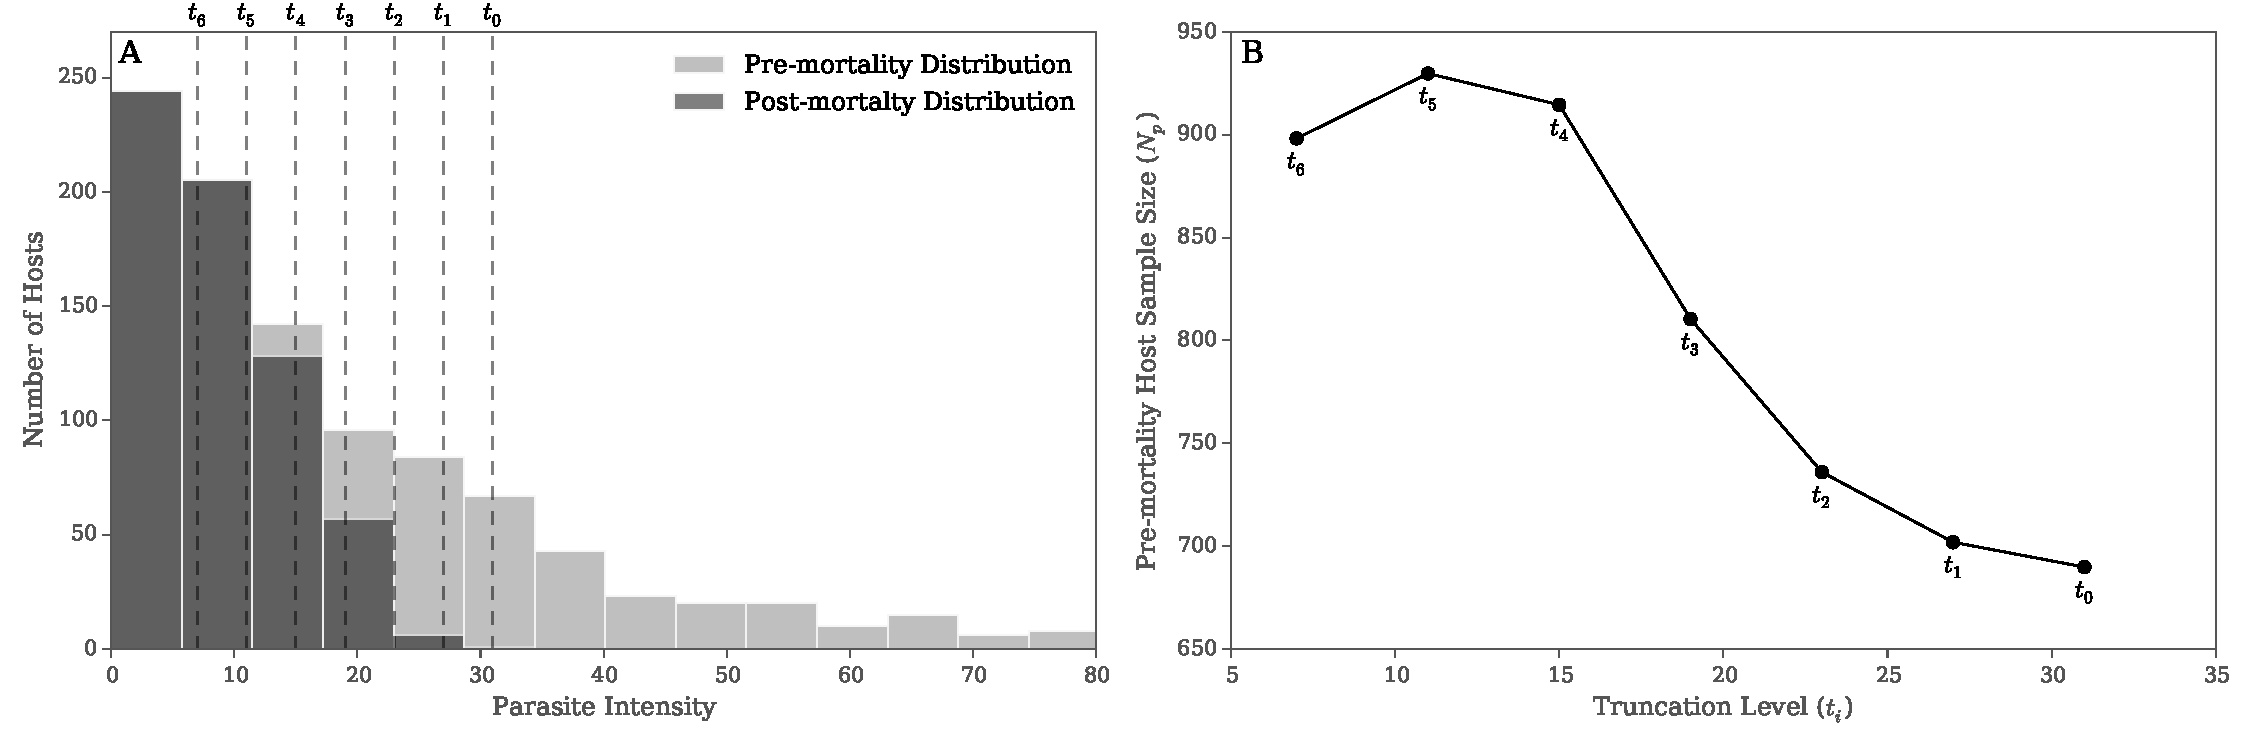
\includegraphics[width=\textwidth]{/Users/mqwilber/Repos/parasite_mortality/results/concept_crofton_method}
    \captionsetup{justification=raggedright, singlelinecheck=false}

    \caption{A schematic representation of the iterative approach of the Crofton Method. \textbf{A)} The light gray shows the pre-mortality distribution that the Crofton Method is trying to estimate from the dark grey post-mortality distribution.  The Crofton Method proceeds by truncating the post-mortality data at different levels ($t_i$, e.g. $i= 0, \dots, 5$) and finding the pre-mortality host population size ($N_p$), pre-mortality mean parasite intensity ($\mu_p$), and pre-mortality parasite aggregation ($k_p$) that best fit the truncated data. \textbf{B)} The parameter $N_p$ is then plotted against the truncation level $t_i$ to determine if a ``kink'' occurs in the parameter values  \citep{Lester1984}. This ``kink'' indicates that PIHM is occurring in the system. In the above example, PIHM is occurring in the system as visualized by the distinct ``kink'' at $t_3$.}
    \label{fig:crofton}

\end{figure}

\begin{figure}

    \captionsetup{justification=raggedright, singlelinecheck=false}


    \caption{A) Five potential shapes for a host-survival functions. In the simulations we used a gradual survival function (dotted line), and moderate survival function (dashed line), and a steep survival function (solid line). The linear and immediate survival functions represent two potential extremes that we do not include in the simulations. For each of these survival functions and the parameter combinations described in the main text, we tested the Type I error and power of the Likelihood (Like.) Method and Adjei Method. B) Gives the Type I error of each method over a range of pre-mortality sample sizes with a pre-mortality mean parasite intensity ($\mu_p$) of 50 and pre-mortality parasite aggregation ($k_p$) at 0.5. The red line shows the pre-set significance level of 0.05. C) Gives the power of each method for detecting PIHM over a range of post-mortality sample sizes for $\mu_p = 50$ and $k_p = 0.5$.  In general, the Likelihood Method has higher power and lower Type I error than the Adjei Method.  See the \emph{SI} 3 Fig 1 - 3 for Type I Error and power results for all parameter combinations.}

\label{fig:question1}

\end{figure}

\begin{figure}
    %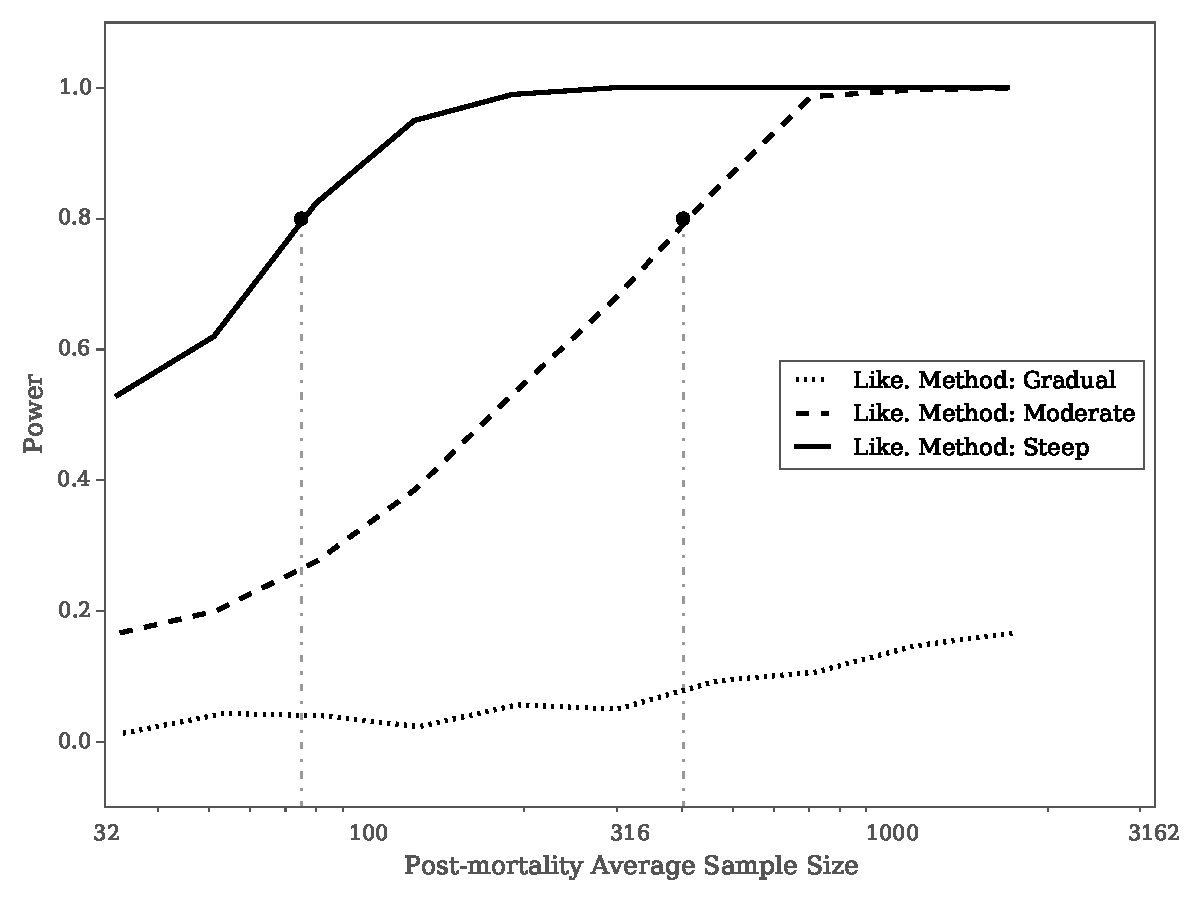
\includegraphics[width=\textwidth]{/Users/mqwilber/Repos/parasite_mortality/results/figure3_for_manuscript.pdf}

    \captionsetup{justification=raggedright, singlelinecheck=false}

    \caption{The power of the Likelihood Method (Like.) to detect PIHM for gradual, moderate, and steep survival functions when all four parameters $\mu_p$, $k_p$, $a$, and $b$ were jointly estimated. The curves were generated from 500 simulations for 10 pre-mortality sample sizes, $N_p$. The vertical, dotted-dashed lines indicate the sample size at which the power the for the Likelihood Method with steep and moderate survival functions is 0.8 (75 hosts for steep functions and 402 for moderate functions). The Likelihood Method with a gradual survival function never has a power above 0.8.}

    \label{fig:real_power}

\end{figure}

\begin{figure}

    %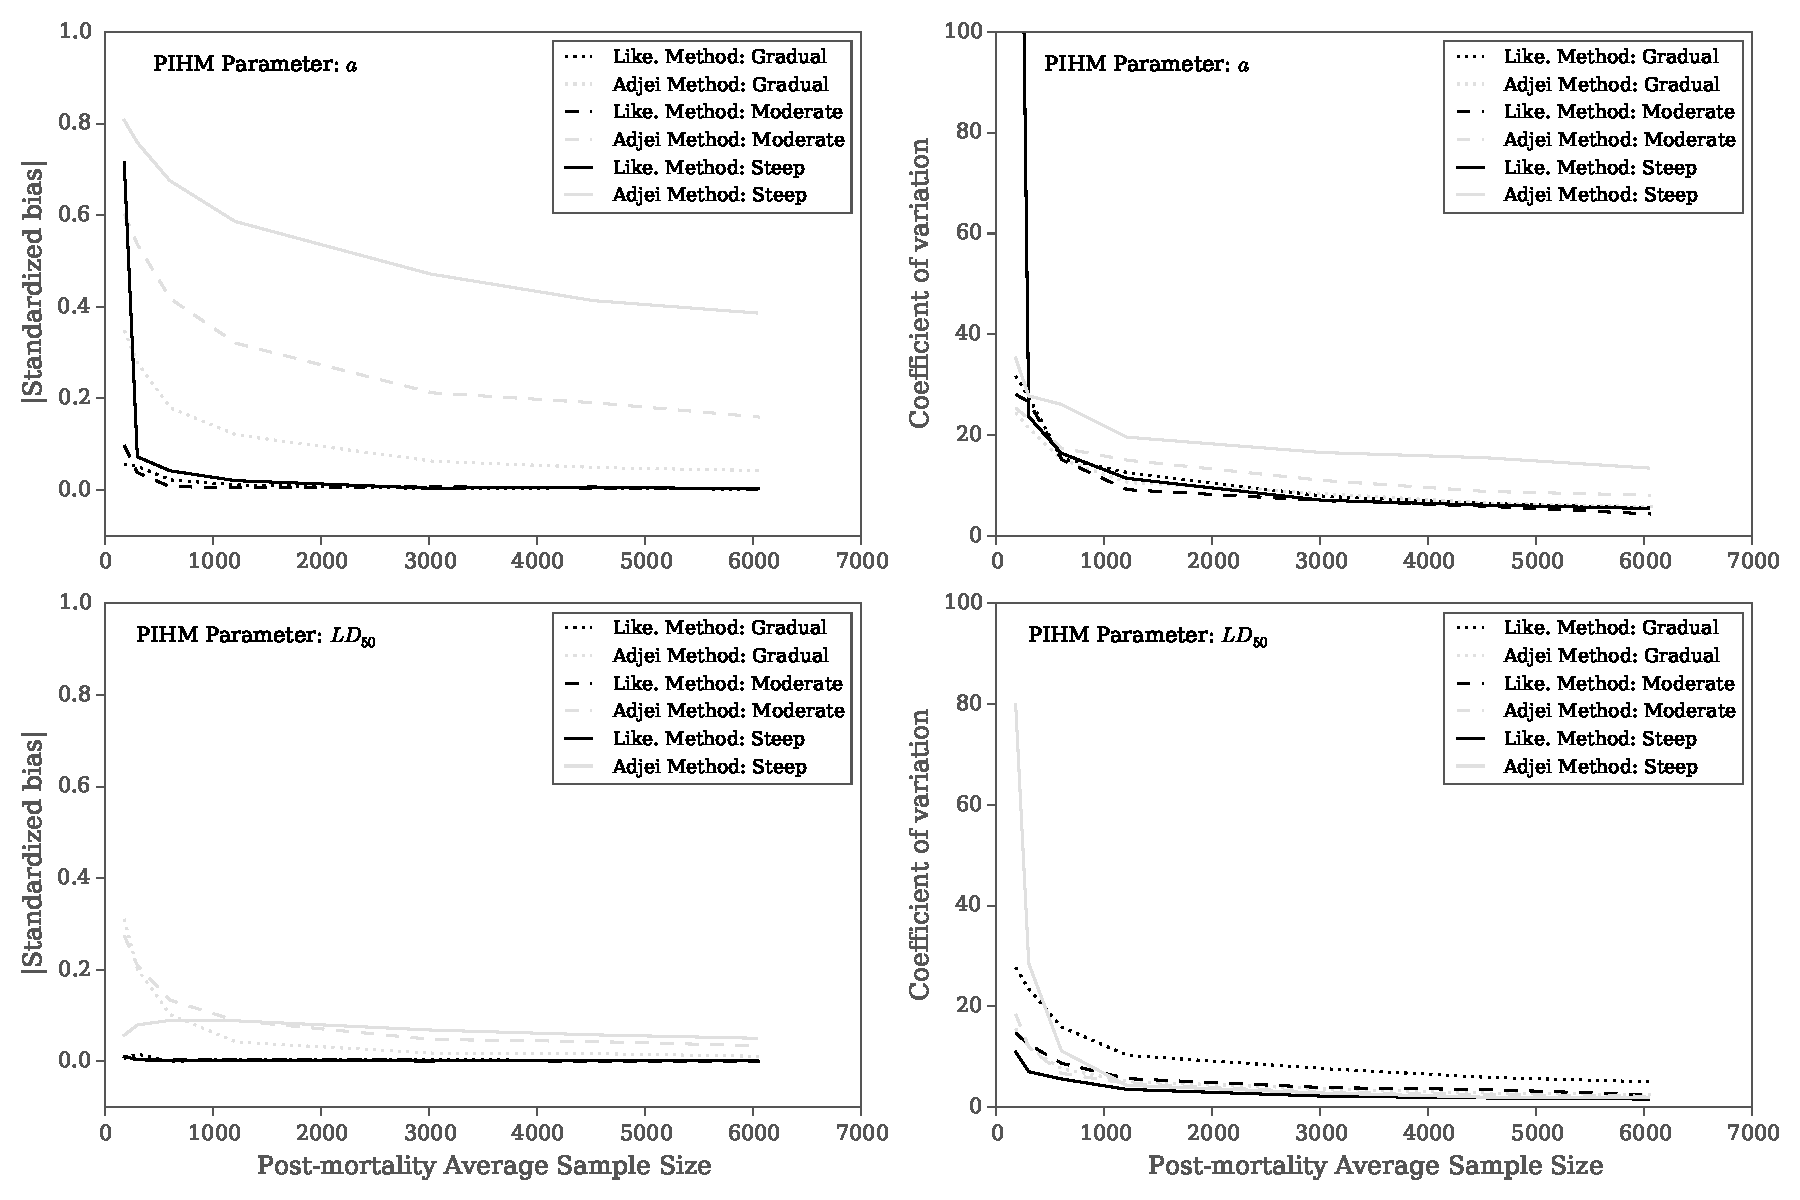
\includegraphics[width=\textwidth]{/Users/mqwilber/Repos/parasite_mortality/results/figure2_for_manuscript.pdf}

    \captionsetup{justification=raggedright, singlelinecheck=false}

    \caption{Bias and precision (coefficient of variation) for the Likelihood Method (Like.) and Adjei Method estimates of the $a$ parameter and the $LD_{50}$ of the host survival function based on simulated PIHM data over a range of post-mortality sample sizes.  As the coefficient of variation increases, precision decreases. The pre-mortality parameters for this simulation were $\mu_p = 50$ and $k_p = 0.5$.  The figure shows the simulations for three different host survival functions (gradual, moderate, and steep), each with the same $LD_{50}$.  Bias and precision results of $LD_{50}$ and $a$ for all other parameter combinations can be found in \emph{SI} 3 Fig 4 - 9.}

    \label{fig:question2}

\end{figure}

\end{document}

